\runningheader{Oppgave l), frivillig}{}{Side \thepage\ av \numpages}


% ********************************************************
% oppgave l) 
% ********************************************************  
\item[l)]
  Kopier modellen fra deloppgave k). For å se forskjellen mellom to aktuelle
  interpolasjonsmetoder, skal du kopiere
  den allerede eksisterende {\sf 1-D Lookup  Table}-blokka og
  legge den i parallell med den første som vist under.
  \begin{figure}[H]
    \centering
    \hspace*{0mm}\scalebox{0.8}{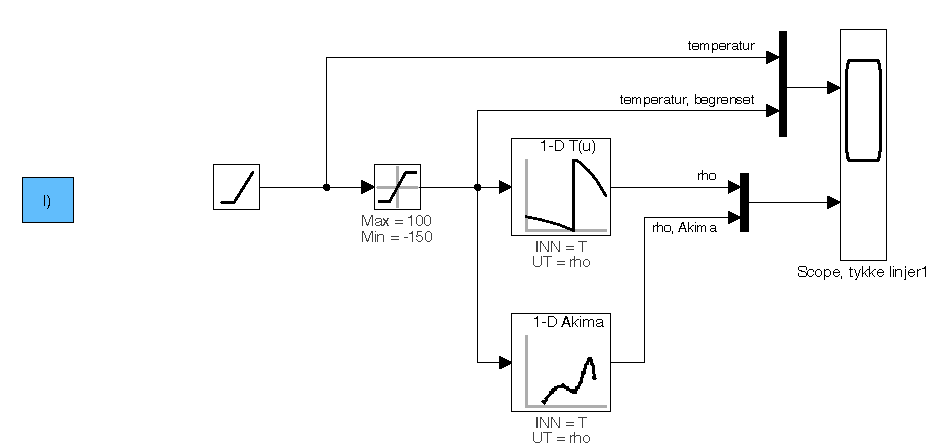
\includegraphics{2l.pdf}}
  \end{figure}
Endre deretter interpolasjonsmetoden i den kopierte blokka
  til  \dbox{\sf Akima   Spline}, sjekk
  {\color{blue}\href{https://en.wikipedia.org/wiki/Akima_spline} 
    {https://en.wikipedia.org/wiki/Akima\_spline}}.
  {\color{red}La simuleringstiden fortsatt være 25 sekund.  }

Simuler modellen på ny, forstørr et område rundt der hvor tettheten er
$\rho{=}1000$, og vis at du får resultatet vist under.
  \begin{figure}[H]
    \centering
    \hspace*{0mm}\scalebox{0.34}{\includegraphics{fig_2l_zoom.png}}
    \caption{Resultat som viser forskjellen på
      interpolasjonsmetodene.}
    \label{fig:akima}
  \end{figure}

  Hva viser resultatet om forskjellen på interpolasjonsmetodene?